\begin{poetry}{Primavera}{Sasha Orr}
It's one of my favorite times of year.\\
Knobs on branches, faintly green and pink,\\
on the crest of burgeoning petals\\
spindle out into florid air,\\
blown against the white-blue sky.\\
on my breath is a wish that this\\
Spring I will know. The baby birds,\\
fallen or flying, will tell me.
\end{poetry}

\begin{poetry}{On our [trans]formations}{Nick King}
It is me who twists your words.\\
It is me who melds your tongue\\
With my body. Questions are stirred\\
With my voice, lies are strung.\\>

My body is your battlefield,\\
My name your target desires,\\
And with you it will be revealed\\
That all we all are liars,\\>

The ones who grow into new,\\
The ones who shed the old.\\
My body is not split into two.\\
My body is made of gold.\\>

Among you, we shine the most bright.\\
After everything, we kindled our own light.
\end{poetry}

\begin{poetry}{Growing in Love}{McKaila Bushu}
Love is sacrifice, love is pain, love is beauty, love is the blossoming fallen fruit on a diverted lane.\\
Sweet and savory, kills and grows, we use “falling” in love as the term but why not growing in love because that's how it's shown.\\
Grows in time, grows in fuming flame, my love, our love, so big and bright, something never to be tamed.\\
As beautiful as the bright orange and red leaves on the autumn tree, as the safe warm crisp air when I'm near you because with you I am forever free.\\
It's peaceful and calming, something I never want to let go, just as perfect and meant to be as Prince Charming and Snow.
\end{poetry}

\art{\notitle}{Grace Woodburn}{p28.jpg}

\begin{prose}{essay}{First Steps}{Makayla Alder}
I can imagine. Not yet knowing how it felt but seeing everyone around you do it without thought. Your height is a mystery. You have never stood on the bottoms of your feet. Is that why they are still so soft? You have never felt a rock get stuck to the humidity of your sweaty toes or seen the small imprints they leave behind. You have never burnt your bare feet on the pavement caused by the beams of the sun. How do you know if your shoes are too big or too small? How do you know if they'll give you blisters or if they give the arch of your foot enough support? How do I know? You have to stand in them to know. So you try for weeks, months. It's just like when you learned to hold your head up. For the first few tries, your legs won't be strong enough to even propel yourself from the floor. As you hold the edge of the wood-stained TV stand with your tiny hands, you use your arms to pull yourself off the ground. Your legs sway side to side as you get used to the new feeling, the new view. Your glance is steered towards the TV playing your favorite nursery rhyme. Do you know you're standing right now? You're doing it. Your guardian pulls out their camera and records the moment, the first time and the only first time. Shouldn't they be sad? You're growing.
\end{prose}

\begin{poetry}{Crippled}{Jesse Looney}
How long until it breaks me,\\
snaps my spine over its knee\\
and rolls me off onto the hardwood,\\
crippled, never to walk again?
\end{poetry}

\begin{prose}{essay}{Cruel and Unusual Punishment}{Keyton Castillo}
When I was twelve years old, I remember that I was a calm guy and I liked to stay at home, and also I never liked to go to parties. Perhaps this may sound weird to you, but I had many close friends with whom I grew up. My friends and  I used to play soccer.  I was lucky to meet them and stick with our friendship. However, here's a detail: my friends were popular but I was not. As my friends were popular they used to know the girl I was in love with. Her name was Stacy, but I knew she would never give me a chance.\par
I used to live with my father in Costa Rica, the town's name was San Rafael de Alajuela. My father has always been a serious and strict man. He was the kind of father who gave you some occasional permission to do some things. My father hasn't been lucky at all with women, and I believe that I inherited that from him. We lived in a small house with two doors, one on the back and one on the front. I remember that there were more windows than doors. We had a small bathroom with a window that I used to escape. I used to call this window my special window. My father didn't know anything about how I used this window. If he knew he would probably remove it. I was escaping through this window everytime that I wanted to go and play soccer with my friends, but this time the reason why I was going to escape was going to be different.\par
One Friday after school, my friends were planning to have a party on Saturday at 7 p.m. They decided to invite me because they knew I was in love with Stacy and she would be at the party as well. How in the world would I miss this opportunity to just see her! But there was one challenge: gaining my father's permission. I knew that my father wouldn't let me go to that party because he was strict, but I wondered if I could do something to make him let me go. So, I decided to clean the whole house. I washed the dishes, bathed the dog; I swept the floor, then I mopped the floor; even that day I didn't eat anything so as not to dirty the dishes so when my father arrived at the house he would see the house clean. \par
On Saturdays, my father used to go to a bar after a hard working day in construction. It was 4:30 p.m. when my father arrived home. He saw that I did a nice job with the house and that I had cleaned the house very well. He wrinkled his eyes and said “good job, Keyton.” Seeing him smiling and happy, I thought, `well, now is the time to ask him for permission.' But I couldn't summon the strength. I was still too scared of his answer. I was so scared that I saw the door of his bedroom and it was as if it turned to rock, and in the rock was a dark hole, the rims of it lit by a fire surrounded by dangerous neanderthals, as if the door said “Welcome to the Cave.” Nonetheless, I somehow summoned the courage and blurted out: “Would it be alright if I went to Jose's house for his party tonight?” But, just as I feared, his answer was a resounding “no.” \par
I felt very upset, but I asked myself,  `if I escape to go and play soccer with my friends, why would I not escape to go and see the girl I'm in love with?'\par
I decided to take a big risk. I put on the best clothes I had, and, as I had done many times, I climbed out my secret window.\par
I arrived at the party at 9 p.m. I said hello to everyone, but I was looking for a specific person, and I found her. I didn't find her the way I would like to find her, because she was already talking with somebody else. But I was thinking that maybe he just might be a friend. As the time passed it became more and more obvious that everyone was enjoying the party except me. It was almost 1 a.m. and the party was going to end when I saw my chance: I would offer to walk her home and then come back. When I approached her, she asked me if I could bring her something to drink and of course I did.  Even though she only talked to me just to ask me for a favor I was elated, and I said to myself, `this is the moment, I have my girl, I don't care what my father is going to do to me, even if he is going to hit me, I don't care, that's not going to hurt me, because I have my girl.' I was having a picture in my mind where after the party I was holding her hands, and telling her how much I loved her, and after that I saw myself kissing her, having one of the best moments in my life with the girl that I had been in love with.               \par
But my dream, as exhilarating as it was, didn't last long. As soon as I returned with her Coke, I saw her kissing the guy who she was talking with. I didn't know how to feel, but the only thing I knew was that the big risk I took was worthless. The worst part was that the guy who she was talking to took her home, and I didn't want to think what could have happened on the way, but I knew that my heart was broken. My friends laughed at first but then they told me, “Don't worry Keyton, there are more girls on the earth than stars in the sky.” \par
You probably think that the situation could not have gotten any worse, but it did. Me and a friend were the last ones awake, telling some jokes about our childhood, and just when the situation started to get a little bit better for me, there was a cop behind me. He was looking for me because my father was scared, he thought that I was lost. The cop took me and dropped me to my father's house. The only thing I knew was that my father was going to destroy me. When I arrived at my father's house he was looking at me. He didn't do anything to me, but I knew from his look that I was in trouble. \par
The next day, on Sunday, he woke me up and told me that I had to work with him. He asked me what happened the day before, and I just told him the truth, and explained it all to him, because if I didn't he would destroy me. He was really mad at me, but when he heard the story he didn't get any madder, he just laughed and laughed. His laughter at my expense felt better than his disappointment and rage, so, all in all, I thought that that Sunday was going to be a good day, that I would be allowed to work and forget about what happened. But no, it only got even worse!\par
My father and I ended up working at Stacy's mother's house. I didn't know that he and Stacy's mother were friends. To say the least I didn't like to be there, but I knew that I had to because I had to fulfill my punishment.
\end{prose}

% 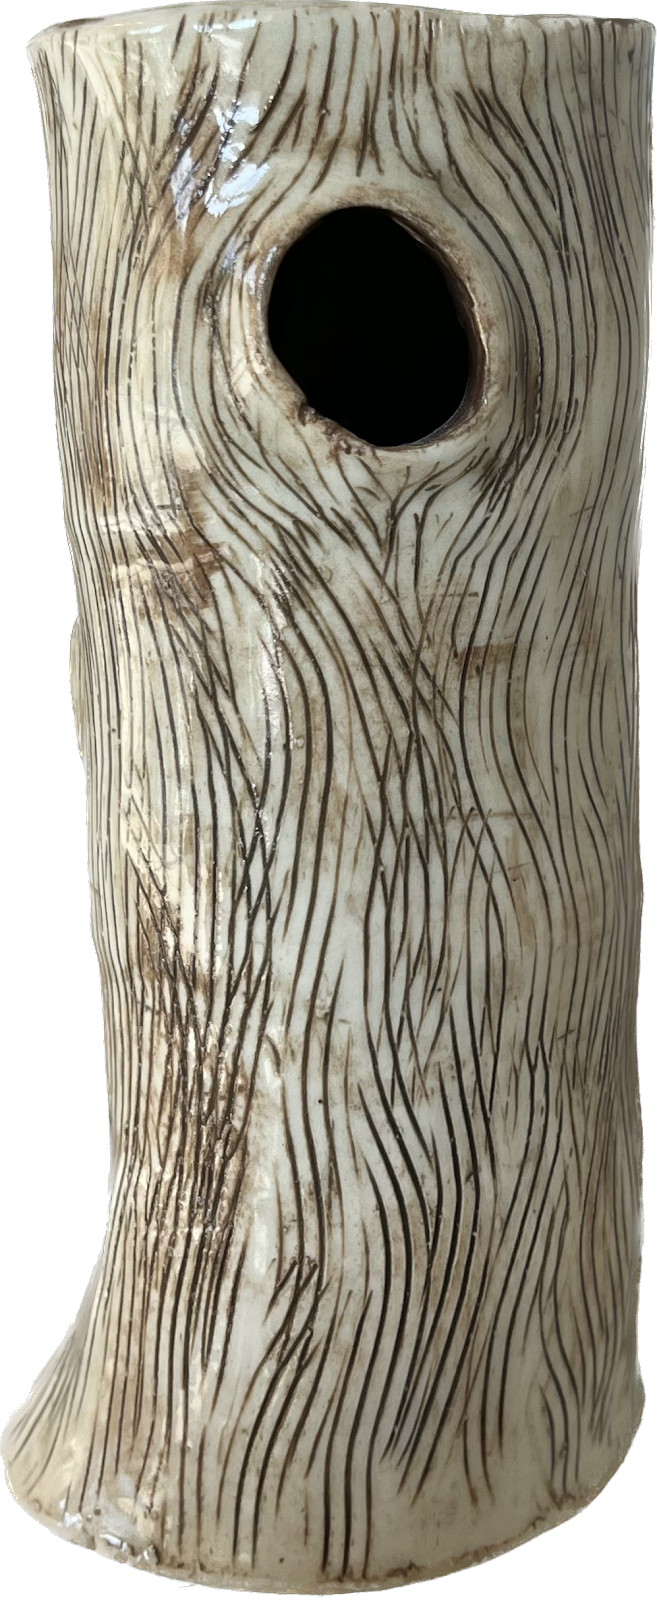
\includepdf{./images/p43.png}

\art{\notitle}{Jasmine Bravo}{p43.png}

\clearpage
\pagestyle{footerpage}
\begin{justify}
    \begin{center}
        \centertitle{\Large{\notetitle}}
    \end{center}

    \vspace*{\baselineskip}

    \noindent{}Immediately following this brief essay,
    you will encounter a series of poems,
    four of them in fact, that all share the
    title “Twerk,” despite being composed by
    different poets. Farther along in your
    journey through this anthology, you will
    encounter another series of five poems,
    all entitled “Syringe,” penned, again, by
    various authors. Betwixt these sections,
    you will come upon a third grouping,
    each poem entitled, oxymoronically,
    “Exquisite Corpse,” and lacking an attribution.
    Each of these exercises are the
    product of the Creative Writing Club's
    generating and experimenting with what
    practitioners of the craft call \textit{nonce forms:}
    poems that adhere to formal criteria created
    by the poet or poets themselves. The rules of
    form can be dictated by a wide variety of
    poetic elements, such as meter, syllable
    count, length, rhyme, and even time limits. Here
    is a brief explanation of the nonce forms
    adopted in this inaugural issue of \textit{Monument}
    (formerly \textit{Inkblott,} formerly \textit{The Thinker} etc. etc.)
    
    \begin{center}
        \centertitle{\large{Tea Bags}}
    \end{center}
    
    \noindent{}The poems entitled “Twerk” and
    “Syringe” are what we call Tea Bags.
    The form is influenced by two primary
    poetic traditions: the acrostic poem
    and syllabics; however, the former has
    been modified. In a typical acrostic poem,
    say the ones you composed in early elementary
    school, one would traditionally write one's
    name or a word down the left column, and
    then use the letter that begins each “line”
    to write a word that describes the named
    person or thing. In the case of the Tea Bags,
    you will notice that the word \textit{twerk,} for example,
    is written down the left column, but instead
    of merely generating a word for each line,
    the poets compose a line of poetry. But you
    will also notice that the lines are of
    varying lengths, each adhering to a strict
    syllable count: line 1 is ten syllables,
    line 2 is eight syllables, line 3 six
    syllables, line 4 back up to eight, and line
    5 returning to ten. The “Syringe” poems
    adhere to different syllabic counts but,
    like the “Twerk” series, angle in and then
    back out of their center, which is also, of
    course, one of the reasons for the form's
    name: the poems are shaped like a cheap tea
    bag, specifically the triangulated fold to
    which the steeping string is stapled. But the
    tea bag, or at least tea itself, is also of
    symbolic importance. Most of us are well
    aware of the idea that one can discern the
    future---prophesize---by “reading the tea
    leaves,” or taking a close, deep look into the
    arrangement and lengths of their vegetative
    veins to divine things others cannot, which
    is what poets do. As such, enjoy a few cups
    on us.
    
    \begin{center}
        \centertitle{\large{Exquisite Corpse}}
    \end{center}
    
    \noindent{}The rules, or form, of
    “Exquisite Corpse” poems are far less rigid,
    consisting only of time and ambiguity.
    In the “game,” writers position themselves
    in a circle around the room. Each writer is
    armed with a blank piece of lined paper and
    a pen. To begin, each writer has 30 seconds
    to compose a single line of poetry about
    anything. When the 30 seconds are up, each
    writer passes their paper to their right;
    they then have 30 seconds to add another
    line to the beginning of the poem they were
    handed. But this is where the fun starts.
    When the 30 seconds is up, the second writer
    must fold back the paper
    so that the next person---the third person---
    can only see the line the second person
    wrote. This is where the ambiguity comes in:
    there is never any context beyond the single
    line, phrase, or word visible to you when
    handed the paper. When each paper gets back
    to its original owner after the first or
    second time around, the poems are unfolded
    and read aloud to maniacal laughter, along with
    horror occasionally, shame frequently, and
    tears sometimes. Ultimately, the exercise
    puts on full display the mind's ability to
    discern narrative, to see patterns, and to stitch
    together disparate parts and make a whole of
    so many fragments. We have included four of
    these pieces for your reading pleasure, and
    hope that pulling back the veil on their
    construction does not diminish the strange
    unity that makes any denial of the Muse but
    the fart of a philistine.
\end{justify}
\clearpage
\pagestyle{main}

\clearpage
\setauthor{}

\myindex{poetry}{Twerk}{\string\various}

\poetrytitleandauthor{Twerk}{Jesse Looney}
\begin{verse}
    The scent of Autumn rushes in the door\\
    With crisp yet subtle fragrance that,\\
    Exuded by dead leaves,\\
    Reminds me of impermanence:\\
    Knife which bisects this moment from the past.\\
\end{verse}

\vfill

\settowidth{\versewidth}{Knowingly against you, your leaf has turned.}
\hfill\begin{minipage}{\versewidth + \vleftmargin + 15pt}
\poetrytitleandauthor{Twerk}{Haley Goudreault}
\begin{verse}
    The trees outside, they are rustling softly\\ 
    While inside the wind is not heard.\\
    Every man for themselves.\\
    Run with it until they are all\\
    Knowingly against you, your leaf has turned.\\
\end{verse}
\end{minipage}

\vfill

\clearpage

\settowidth{\versewidth}{To let each other in, look me in the eye.}
\hfill\begin{minipage}{\versewidth + \vleftmargin + 30pt}
\poetrytitleandauthor{Twerk}{McKaila Bushu}
\begin{verse}
    To let each other in, look me in the eye.\\
    When I whisper your name to you\\
    Everything becomes brand new.\\
    Remember my voice forever in your head.\\
    Kill the others so mine forever stays.\\
\end{verse}
\end{minipage}

\vfill

\poetrytitleandauthor{Twerk}{Avery Becker}
\begin{verse}
    `Tis a tale to be told in the crystal\\
    With fingerprints smudged on each inch.\\
    Evelyn's breath fogs white,\\
    Reaching to answer the quest, that\\
    Knowledge before he has already answered.\\
\end{verse}

\vfill

\clearpage

\begin{poetry}{Winter at Dusk}{Jesse Looney}
Accompanied, yet lonely,\\
I stride in the fresh air of a clear head,\\
(though my own is not)\\
in the last glimmer of golden light.\\
No—it is sweet but not quite gold.\\
Gold is rich but the light is hollow.\\
It is the color of bleached beautiful things\\
now lost to memory.\\
Everything is ending, it will all come to an end.\\
Suddenly, the wind is cold and bitter.
\end{poetry}

\art{Flowers in the Shade}{Chloe Lawson}{p55.jpg}

\art{\notitle}{Brooke Duquette}{p54.png}

\begin{poetry}{The Ocean is my Enemy}{Sophia Lee}
The ocean is my enemy\\
\tab{}and is seen by others none the same.\\
She breathes salty air\\
\tab{}and the waves become her pulse,\\
the echo of the souls she kept safe in her cradle of brine.\\

And she shimmers\\
\tab{}amidst the amber light,\\
amidst the drying reflection\\
\tab{}of the fire's gaze,\\
her breath, in tousled updrafts,\\
\tab{}seasons the air with frigid tears\\
and trickles down the crumbling dry earth.\\


But the waves are hushed and put to sleep,\\
\tab{}they break on the rocks and ripple.\\
Foam crests lace through the hues\\
\tab{}and she rolls higher into the steep.\\
She whispers\\
\tab{}and only I hear.\\

The ocean is my enemy\\
\tab{}for I envy how one could hide\\
bitterness\\
\tab{}in the sweet cradling sound of death.\\
But envy is oftentimes short-lived.\\
\tab{}Her pulse quickens into drafts\\
and her whispers\\
\tab{}become cries for help.\\

\end{poetry}

\begin{poetry}{Revenge}{McKaila Bushu}
Pain inflicted by the hands of who you don't expect\\
and you still there in utter disbelief.\\
I hate you, why? Why me? Why this?\\
You should suffer.\\
You need to feel this killing pain,\\
But, hey, maybe it's making me tougher.\\>

I wanted this to be perfect, perfect us, a perfect puzzle piece, one\\
that is magic and beautiful.\\
I thought you were with me and it was us,\\
I never would of thought this to be the outcome when we met,\\
but now I've been wrong;\\
I have found my new target.\\>

The plan set in stone, ready to be executed.\\
Why does this feel weird, feel wrong?\\
If I do this will I be the one forever gone?\\
Once this is done, you and me are dead, we have a clean slate\\
but then you kill me once again\\
and that's when I realized I'm always\\
the one meant to get hurt in this story.\\
That's my fate forever.
\end{poetry}

\begin{prose}{fiction}{Moth \& Flame}{Avery Becker}
A moth flutters drunkenly toward the porch light. Every few seconds it seems to be jerked down before rising up again as if, just for a moment, it forgets how to fly.\par
I know what's coming next, but I wince anyway when the moth reaches the light. Having caved to its desires, it gets singed and falls to the ground in a crumple of soft cream and brown whorls. It's a scrap of tissue paper, resting there on sun bleached weeds.\par
The porch light winks off.\par
“Psst! Caleb!” A call from the other side of the fence, which I can't see in the dark but can picture with perfect clarity. There will be tufts of copper hair peeking over weathered gray boards, stormy eyes with flecks of blue. And a grin. \par
That grin is for me what the porch light is to the moth. \par
I rise, the seat of my jeans cold from the brick steps, and move to the side of the yard, the soles of my sneakers grinding the fallen moth into the dirt as I go. When I vault over the fence, I hardly have to think anymore, the motions ingrained in something deeper than memory, something intrinsic. \par
The girl with copper hair lifts a lighter to me the second my feet hit the pavement. I shake off the jolts of electricity thrumming up my calves from the impact.\par
“Why didn't you just bring a flashlight?” I ask this every time.\par
The girl, Mara, only smiles, the contours of her face sharpened by the flickering glow. She slips her free hand into mine. We really shouldn't be doing this again.\par
“Are you sure—” I begin, my voice raspier than normal.\par
“Caleb,” she whines, the word pulled between her teeth like bubble gum. “It'll be quick.” \par
It always is, I guess.\par
I can almost pretend that Main Street is silent at 3 am. Of course, there are dogs barking a few streets over, the clatter of a trash can lid toppling off, the pop of glass exploding off pavement. But these are just the sounds of home, so familiar they fade into the background and nearly into silence. I'll miss it when I move to the city, when I'm surrounded by sirens and shouting. An environment just like this but with a manic gleam in its beady eyes.\par
Beside me, Mara's bathed in orange from the streetlights, lashes dark on her cheekbones when she blinks, lips pulled into a playful smirk. She catches me looking at her and pushes her shoulder into mine. I freeze when her skin brushes against my thin long sleeve, the way I have for nearly seven years. \par
“You really didn't think I'd let you spend your last night all alone?” she asks, smiling in that way that always makes my stomach work itself into knots.\par
I shake my head, not trusting myself to speak. \par
“Just one last run,” she begs.\par
One last run. She knows I don't need the money. I've worked three jobs this summer, which she would know because she skipped nearly half of summer school to bring me soggy sandwiches she got from God-knows-where. How she spent her own summer beyond that, I don't know. I can only assume she was hopping between houses, any house that wasn't her own. On nights we didn't hang out, I'd often see her stumbling out of side yards I didn't recognize in the morning, rubbing bleary eyes and smiling at me shakily. \par
No, she isn't doing it for the money. She just wants one last night. Don't I?\par
“Where to, then?” I ask, caving, bending to her light. “The usual?”\par
“Oh Caleb,” Mara sighs, clasping her hands to her chest and pretending to swoon. “No one knows me like you do.” \par
I look away at her flirting, which isn't anything new. She thinks she's embarrassing me, but it's not quite that. I want it to be real so badly that I'm afraid one look in my eyes will give everything away.\par
I've spent over half a decade in the wake of her lightning, the first hand she reaches for but never the last. Just because she's the only one worth fighting for in my life, doesn't mean I'm the only one in hers. Why would I give myself up now?\par
We lapse into silence again, sneakers hitting the pavement in a rhythm that's more familiar to me than my own heartbeat. \par
Tonight, I can't stop myself from watching her. The baby hair curling under the hem of her hair, right where her neck and shoulder meet, the twin freckles nestled into the smile of skin on the back of her elbow.\par
Every breath of air between us is a chasm.\par
“So,” she says, turning, and I think she's finally caught me. But all she says is, “Chicago.”\par
“Chicago,” I agree.\par
“Aren't you excited?!” She flips so she's walking backwards on Main Street, holding my eyes. “You've wanted to get out of here for forever. You'll have an apartment and a roommate and classes. Classes,” she teases. “With professors.” \par
“You have professors,” I say, rolling my eyes in fake annoyance. She's the one that's wanted to get out of this town since middle school. I've just always wanted to be wherever she was. \par
But I'm the one with the scholarship, and she's not.\par
Mara snorts. “Yes, me. A student. All I want to do is stay out every night, try new foods, see new places, take the subway…”\par
“It won't be any different than here. Just a little more noise and traffic,” I say, suddenly annoyed.\par
A shot goes off in the distance, and I flinch slightly, despite the commonality of it. “See? There'll be ten times the amount of that in Chicago. You could never walk the street like this.”\par
“Yes, I could,” she argues. “And you will. You're gonna be out at night all the time.” \par
“Not at 3 am.” \par
“Yes at 3 am. Going to parties, bar hopping…” she smirks. “With a date.” \par
My stomach lurches. \par
“Caleb?”\par
When I don't respond, she turns so she's walking beside me again. “You're the luckiest guy in the world, going to Chicago. You can't waste it. You can't waste it.”\par
I'm surprised by the vigor in her voice that's almost tipping into anger, but I don't know how not to waste Chicago. I don't know how to live without Mara. She does enough living for both of us.\par
“I'll try,” I say.\par
She stops us under one of the working streetlights, raising an eyebrow at me. \par
“You'll try?” she scoffs and I'm worried I've blown her good mood. “Caleb.” She looks me in the eyes, and I want to kiss her. \par
“I promise,” I lie, turning from her and walking again. When I glance back, she's still standing here, arms limp at her sides. For a moment she seems so small. \par
But then the air shifts and she's back at it again, the light from the streetlamp nipping at her heels like a stray dog as she bounds forward. \par
“We're here,” she says, and I must be imagining the crack in her voice.\par
Digham's Convenience looks the same as it always does: stiff, belly-up cockroaches rocking in dusty windowsills, panes of glass smudged with yearning fingerprints, and a red “closed” sign hanging lopsided from the window in the door. And yet this time, everything feels different.\par
“Ah!” Mara says. “Home, sweet home!”\par
I glance up and down the street, but no one's there. No one's ever there. It's just me and Mara. Mara and me. \par
“Ready?” \par
Mara hovers by the door, fingers rooting in one of her pockets for her lock picking set, which is probably tucked deep beneath a lighter, a pack of cigarettes, and a million other objects that always make her cargo shorts sling heavy around her hips. \par
At my nod, she presses the newly procured lock set into my hand and gestures grandly to the door, winking. “It's all yours. The last time.” I know better than to argue.\par
But when I put the tensioner into the lock, something feels off. It's a change in the air, a chill that wasn't there before. I glance behind me at the street, but it's still empty. \par
“You okay?” Mara asks. I nod dumbly. \par
There's always a sense of danger effused around Digham's. It's why Mara chooses to come here. Everyone knows that one of these days Old Man Digham will crack, that he'll finally have enough of the teenagers that break into his stores on dares and taunts. Just last week, a junior from our high school nearly got his foot blown off. \par
When the lock gives way, I swing the door open, but don't take a step forward. The only light comes from the corner where the humming fridges cast panels of flickering fluorescence onto unswept floors.\par
Mara slips her arm through mine, warming me and making me shiver at the same time. “Your bounty awaits.” \par
“We don't have to do this.”\par
“I want to.” Her eyes gleam in the dim light. “C'mon, Caleb. For me.” \par
There's no way she knows that I would never be able to say no. That when it comes to her I don't even have a choice.\par
“Fine,” I say, and close the door as silently as I can. “Let's just make this quick.” \par
Mara floats to the cash register, grabbing a Snickers and sticking it into her cargo shorts. \par
“How about fifty,” I say, as she works on the register's lock. It's a compromise on our normal twenty dollars each, never enough that anyone would notice. “For the last day.” I know she would insist anyway. \par
“Hmm…” She smirks as she pulls a paper grocery bag out from under the counter. My heart sinks.\par
“Mara, what are you doing?” \par
I duck behind the counter, and she's jittery with excitement as she lifts stack after stack of cash bound with dirty rubber bands, settling them reverently into the bottom of the bag. It is not the lack of morality that scares me, that's never been there. It's the way she's staring at the money like it's already hers.\par
Despite how often it happens in my dreams, I'm certain that she's never looked at me that way before. \par
A creak sounds from a far corner of the store, and I flinch. “Did you hear that?”\par
“It's a rat. C'mon, Caleb.” Her voice has an edge to it that I'm always surprised to hear, but still my hands twitch with the desire to pull the bag from her grasp.\par
“Let's just go. You've got plenty.” \par
She glances sharply at me, and I nearly shrink back. I hate it when she looks at me like that. Like I'm a stranger. \par
“I'm gonna do this.” Her voice is rock hard. “Don't try to stop me Caleb.” \par
“Okay, okay,” I say, reaching toward the cash to help speed up the process. “Let's just be quick.”\par
Crack.\par
I don't feel the bullet the instant it makes impact with my side. \par
One moment I'm standing and the next I'm flat on my back, noticing the gray light in the grimy convenience store, staring at the cracks in the ceiling, a ringing in my ears.\par
Cash that wasn't bound is falling like rain, over my eyes, sticking to my lips. \par
It was all there. The feeling of wrongness in the air, the creak from the corner, Digham's bad eyesight, his rifle that everyone knows that he keeps hanging above his bed on the second floor of the store. \par
Mara. \par
I lift my arms above my head to feel her, and black rings my vision from the effort. \par
“Mara!” I choke out, my voice breaking. Everything goes watery and maybe it really is raining in here, maybe a storm leapt from her gray blue eyes. \par
There are her sneakers, and my fingers draw arcs of red as I scrabble to catch hold of her. Blood is sputtering in my throat, so I turn my head to the side to spit it up and some of it catches on her laces. She steps back, out of my grasp. \par
The hair on my arms rises.\par
“Get out of here, you little punk!” I hear rather than see Digham limping into the room and his voice, like metal grinding into gravel, seems to come in and out like a radio. “Serves your lot right, breaking in here all summer! And take him too, he's bleeding all over my floor.” \par
A jab to my ribs with his cane sends me onto my side and I groan into the concrete, eyes slitting around the pain, a feeling so indescribable I can only compare it to my desire for Mara.\par
“Leave the money,” Digham barks. \par
Gritting my teeth against the agony, I glance up at Mara. Her stance is certain, skinny shoulders thrown back, hair curling with sweat, and despite it all, she's more beautiful than I've ever seen her. A tempest.\par
Digham shuffles and I assume he's bringing his rifle up to his shoulder. “Now, girl. Before I change my mind and shoot you too.” I feel him tapping his foot through the floor. “Clean this mess up.” \par
My breathing is ragged now, and I quiver as her sneakers come towards me.\par
“Girl…” Digham warns.\par
She bends down and it's Mara. Me and Mara. Mara and me. She moves closer until my vision is only coming out in copper and blue, cigarettes and faint lighter fluid. She reaches her hands out above my head. Then her lips are on mine, and though I can hardly feel it through the pain, I don't care that I've been shot, I don't care that Digham is standing over us with a rifle, I don't care about my scholarship or Chicago. I'm staying right here. \par
She pulls away and I'm delirious. But her smile is stretched too thin, and when she draws her arms back, there's cash clutched in her hands. My mind whirls, straining to connect what I'm seeing with the flush in my face.\par
Digham scoffs and cocks his rifle, and I realize too late that Mara's dropped the money in her right hand and reached into her biggest cargo pocket. There's a gun that I've never seen before, and in my slanted vision I watch her cock, shoot, and hear the crumple of a heavy body hitting the concrete before I can even blink. \par
“Mara,” I croak, unable to comprehend that she shot someone, because my mind is still lingering on the kiss, what it meant.\par
She bends over me again and comes back with more cash, the horrifying reality starting to sink in like a lead pipe to the stomach, but the physical pain of it doesn't connect with my brain. \par
There's the crinkle of a paper bag and a woosh as she sweeps cash into it. \par
She killed Digham.\par
A numbness is spreading across my limbs and threatening to take me under. I wait for her to call the police, then to kiss me again as we wait, to hold me to her body, to finish the start of this new something that she created.\par
Mara gets to her feet, cradling the bag like it's more precious than a human life. More precious than Digham's life.\par
I'm paralyzed as she steps backwards, right at the rim of my vision. I'm losing her. I'm losing Mara. \par
Black bleeds into the corners of my eyes, and the ache in my chest has widened to a piercing, pulsing animal that's thrashing around inside of me. \par
“I love you,” I manage to get out because I don't know what else to do, blood bubbling on my lips.\par
“I know you do, Caleb.” \par
She leans over me, breath warm on my cheek, and my eyes flutter closed. Then I feel the cold metal of the gun as she slips it into my open palm.
\end{prose}

\art{Psychotic Trip}{Hannah Desjardins}{p40.jpg}

\begin{poetry}{Raw}{Sasha Orr}
Just soft enough to draw blood,\\
just harsh enough to pierce the skin,\\
that inimitable sensation.\\
Had you felt that clawing need too?\\
Did you feel the soft pulse run through me as\\
you tore in? Can the scope of all that is human\\
be surmised in a single act?\\
The need to feel, relentless, no pulling back.
\end{poetry}

\begin{poetry}{Lovely}{Avery Becker}
Here's something to ponder:\\
perhaps loveliness is not a measure of perfection\\
but the contentment of a moment.\\
Perhaps it is a beauty felt and not observed,\\
the certainty of it tangible.\\
Maybe it's the stripping of aesthetic,\\
the vulnerable, unseen moments at the core.\\>

To illustrate:\\
She is alone in the car, driving home in the dark by the lake.\\
Her awe of life astonishes her.\\
It's this movement,\\
bound by the sunset, then the stars.\\
The lake is beautiful this time of night\\
the houses across the glittering water,\\
lights reflecting a hundred other lives.\\
But she is her own.\\
In this moment it is \textit{such a lovely life}.\\>

If you were there\\
you would see her breath on the windshield like a fluttering thing,\\
a warm shuttle in the cold dark,\\
suspension between what was before and what will come but not concern.\\
She will always long to be held above herself,\\
to observe what she thinks is the loveliness of perfection\\
but is really just this moment, this lovely moment\\
in February driving by the lake.
\end{poetry}

\art{\notitle}{Melody Brien}{p2.jpg}

\begin{poetry}{Brick to the Chest}{McKaila Bushu}
The feeling of a brick to the chest,\\
why do I go through this? It feels like a constant test.\\
My heart aches at the thought of it all, begging tightest back and forth,\\
my head's about to hit the wall;\\
a smile on my face while the little me in my head is pleading for help;\\
one wrong move and she's gonna melt.\\
Can anyone see how much pain is in my heart, in my head, in my body;\\
that strong pain, the pain of when we are apart?\\
Let them in. Let them hear how much you have to say.\\
They say do it and the pain will magically go away.\\
It's a release, it will help.\\
They say so many things in my ear, hoping to understand my pain.\\
It's starting to drive me insane!\\
Why can they put it into words and I can't?\\
Other people are happy and healing, makes me want to get a brain transplant;\\
maybe then I won't feel the pain, feel the torment from my brain\\
telling me it's not going to be ok and put me in the right lane.\\
Am I crazy for feeling this hurt?\\
I mean people go through worse and make it out fine,\\
maybe I'm being dramatic,\\
maybe all of this is a waste of time.\\
So I'll take the brick and put it back in the wall\\
and sit down and listen to you all\\
like a brick to the chest.
\end{poetry}

\begin{prose}{essay}{First Love}{Ava Vasquez}
    You're young, you idealize the “picture perfect” relationships on TV.
    \textit{The Notebook, Titanic, Heartstopper,} etc. You become a hopeless romantic, searching for love in all situations. But remember: you're young. Do you really know what love looks like? Or is it the actors who are forced to press their lips upon each other for their next check? Those butterflies you're feeling, \textit{that high,} the light their smile emits as soon as they walk in a room, your new \textit{desire} to walk the long way to class in hopes to bump into them, is that real? You decide to try love, what could go wrong…right?\par
	Now you're in your first relationship. Your day doesn't start until that “Good morning! <3” text. But don't let it be “gm,” “good morning,” or “morning,” because now your “morning” is ruined. Once you see that heart, enthusiasm, that hug before class, anything is possible. You feel everything with them, but not a thing when it begins to get hard. So why is it when the love grows stronger, the pain hurts worse? The more you fall in love with “your person,” the more you're hurt by them. They show you what being on top of the world feels like—that time they surprised you with flowers, teddybears, took you to your favorite diner, made you soup when you were sick, all of those memories made you feel good; so why would the person you love most hurt you? How could they do all of those nice things and then scream at you for hours, kick you out of their house, and stare at you \textit{emotionless} while you're crying over \textit{their} actions? Is this your ideal love? I guess the movies and shows don't show that part though. \textit{Titanic} doesn't show Rose \textit{desperate} for Jack's love as he slowly ruins her esteem. They don't show the hard questions like \textit{Do you even love me anymore?}. The movies don't show you staying up late at night crying, asking yourself how someone you loved so deeply is \textit{ruining you.}\par
	So it gets toxic, you don't want to leave but know change needs to happen. You wait… and wait… and wait. You're wrapped in the toxicity now. You're checking their location to see where they must be if it's taking so long to reply. \textit{Who's there? Are they single? Make sure they're not flirting with you. Why did you look at her like that? Do you like her?} All while you're still hurting and insecurities form. Who knew love could affect you this much? You're still here though, still together. That's what's important…right? \textit{Loyalty?} So why is it when you check your phone you see that text. You know what text.
\end{prose}

\begin{poetry}{Sweet Tooth}{Jesse Looney}
To what do we owe the pursuit of pain,\\
as when we lever a loose tooth\\
till the piercing prevents us,\\
and yet, unable to bear the ache of relief,\\
we plunge back into pressing,\\
forced to savor the tartness of misery?
\end{poetry}

\art{\notitle}{Devon Buscema}{p53.png}

\begin{poetry}{Adrift in Time}{Sophia Lee}
I was in my head\\
\tab{}wishing in a fountain of my own tears\\
and throwing coins just to watch them sink.\\
\tab{}Young,\\
invisible folds of skin\\
\tab{}and streams of dark rivers,\\
a head of bleeding ink.\\
\tab{}Picking on the dress of a sun \\
petal by petal,\\
\tab{}wishing the final tulle-made skirt told me\\
that it was okay to leave.\\>

Stolen chalk scathed onto the stone floor,\\
\tab{}dolls and puppets\\
and fighting over roles in “House,”\\
\tab{}crying and screaming to seek eyes\\
and stones and pebbles we found in a scar of the earth\\
\tab{}until we realized the world turns to age.\\
We outgrew our clothes\\
\tab{}and outgrew hopscotch\\
as the street crumbled some more\\
\tab{}but always the chalk was stolen and the stones were free.\\>

The world was turning\\
\tab{}and I was not prepared for it.\\
No one warned me\\
\tab{}and no one stopped me.\\
We were all children hopping on one leg\\
\tab{}on the autumn-kissed sidewalks\\
when suddenly\\
\tab{}everyone had ambitions,\\
everyone had motives,\\
\tab{}and I was not prepared for the world to turn\\
so the world left me behind.\\>

And it was both a curse and a blessing,\\
\tab{}for it stowed me away to live in the dark corners of the universe.\\
I remembered that color only comes after black and white,\\
\tab{}that you can draw chalk\\
on the dark cement of the earth.\\
\tab{}And I painted strokes on a blank canvas\\
until I began painting in my head\\
\tab{}and too much for one open soul.\\>

So then there were two,\\
\tab{}screaming in joy\\
and smiling in fear,\\
\tab{}foam swords and ketchup blood,\\
and my heart drinking the saturation of hues like wine.\\
\tab{}He had his sword in my chest, and I pressed mine in his\\
and anything we wanted\\
\tab{}we painted it and engraved it into our heads.\\>

We flew on invisible strings\\
\tab{}and soared too close to the sun\\
and our silhouettes towered\\
\tab{}over the frosted sidewalks.\\
The chalk and stone from the scar of the earth lived through time\\
\tab{}but in one tear\\
the paint washed away.\\>

I was in my head,\\
\tab{}Trapped in my childhood with cold winters \\
and hot summer days.\\
\tab{}Angels in the snow\\
and sand between my toes\\>

He was right behind me\\
\tab{}and had been all this time like a low breath.\\
But by the fountain of my own tears\\
\tab{}I watched a coin sink my final memory\\
and in miracles, my wish came true.\\>

For I closed my eyes\\
\tab{}and never opened them again to leave.\\
I crossed time\\
\tab{}with no arm to hold me back.
\end{poetry}

\art{The Minister's Black Veil}{Julia Santos}{p51.png} % p10 in MONUMENT, SPRING 2023

\clearpage
\setauthor{}

\myindex{poetry}{Exquisite Corpse}{\string\various}

\poetrytitle{Exquisite Corpse}
\begin{verse}
    The snow falls onto the ground as the sun sets into the night.\\
    The owls call, the darkness rises, and the stars light up the snowy sky.\\
    The moon seemed to fall right on the cup the seas formed.\\
    Forever blinding, no more to touch, no more to bleed,\\
    just a husk, a shaft that, stripped, flutters to the floor\\
    like leaves on a path, which fell from something beautiful and whole.\\ 
    I walked with you, brushing fingers like promises of false futures\\
    whose realization is quintessentially impossible,\\
    yet she still remains hopeful, nonetheless.\\    
\end{verse}

\vfill

% \settowidth{\versewidth}{Knowingly against you, your leaf has turned.}
% \hfill\begin{minipage}{\versewidth + \vleftmargin + 15pt}
\poetrytitle{Exquisite Corpse}
\begin{verse}
    Rusted gold, weathering down, eroding in the silver wind.\\
    Light centering to a perfect dapple, illuminating the ground.\\
    Shining from up above, only the gods can see me now\\
    as I kneel at the grave of my father. \textit{Do I wish I could take it back?}\\
    But where grief meets anger, I still feel nothing,\\
    the hollow of a vase, meant to sit, nothing to hold,\\
    but longing and desperation\\
    could never be undone.\\
    A moment comes, a moment goes, forever all, forever one.\\    
\end{verse}
% \end{minipage}

\vfill

\clearpage

% \settowidth{\versewidth}{To let each other in, look me in the eye.}
% \hfill\begin{minipage}{\versewidth + \vleftmargin + 30pt}
\poetrytitle{Exquisite Corpse}
\begin{verse}
    Nostalgia always finds its way back to you,\\
    your scent, the touch of your woolen flannel\\
    Softer than a spoken word\\
    but still louder than everyone in the crowd.\\
    The voice grows louder, deafening the surrounding silence,\\
    and then it stopped.\\
    Silence after the pause, no noise to be heard but forever to be felt,\\
    the shock of it, a wild thing that cannot be controlled\\
    but can be tamed by our past.\\    
\end{verse}
% \end{minipage}

\vfill

\poetrytitle{Exquisite Corpse}
\begin{verse}
    Ill intent causes forever broken trust in the mind of our own.\\
    A circle that once cracked can only be patched with time\\
    like a heartbreak resembling the ache of loss,\\
    figured in the shards of the cracked mirror\\
    whose disparate pieces shall never be decollated,\\
    whose heart will never become whole again.\\
    And though their heart has shattered into small fragments\\
    their head was still whole\\
    but their body done, no more to give but their soul, which was the only thing that felt whole.\\
\end{verse}

\vfill

\clearpage

\art{The Ugliest Creature to Crawl from the Kiln}{Mikaeylla Nardy}{p15.png}

\art{\notitle}{\noartist}{p46.jpg} % p22

\begin{poetry}{Abuse}{McKaila Bushu}
Abuse on my heart,\\
abuse on my mind,\\
may not be seen but forever shown\\
in my words\\
and my eyes\\
and the breaking of my tone.\\>

Hollow like an apple without a core,\\
thoughts piercing like a forever bruising sore.\\
Weak in the mind, you take it when you please,\\
take and take,\\
abuse it,\\
then you leave.\\>

My hurt never seen,\\
being killed, invisible blood,\\
being killed me and wiped it imperfectly clean.\\
Knife to the soul,\\
knife to what feels like a black hole,\\
taken the hope, abused the mind\\
but no one ever knows because everything's beautiful under sunshine.
\end{poetry}

\begin{poetry}{Powdered White}{Avery Becker}
fever haze and snow globe daze\\
smothered sky enslated white\\
i'm upside, inside, downside out\\
swirled around in crystal cage\\>

without a clue, time comes clocking\\
ticks by and tocks me, drawing red\\
spooling out in cotton coils\\
choked by existential dread\\>

as certainty is shaved away\\
by chisels made of snow and ice\\
reality is slurred and blurring\\
slipping world tips into night\\>

pulsing voices multiplying\\
mock me lost in binding squall\\
an avalanche of my confining\\
burning shards of bitter cold\\>

limp, surrendered to the storm\\
numbness claws and nestles in\\
all that's left is hollow shell\\
embalmed in frosted glass again
\end{poetry}

\begin{prose}{essay}{Bath}{Makayla Alder}
When I was young, it was bubbles floating on the surface of the water; playing with the cups from the kitchen cabinets and random objects that were dispersed around the house. I wasn't worried about drowning because you were there watching me. I wasn't shameful about being naked. Now I rarely take baths. I don't like the feeling of the water tight against my body. It feels like I'm being compacted into nothing. I can feel my lungs trying to breathe and the shortness of my breath. I am worried about drowning now, purposefully. What would you think of that? I wish my shortness of breath turned into breathlessness. I wanted to relieve my stress and anxiety by taking a bath, but there's only one way to really relieve it but it's too still here. It's nothing like the beach, where the waves move and crash on their own. Here, the water only moves if I move. There is no sound after the bath is full. My mind is constantly moving and thinking, like a machine that shuffles cards. I want to find something that can silence my mind, but my mind is the loudest thing in the world though no one else can hear it.
\end{prose}

\begin{poetry}{Autoerotic Asphyxiation}{Jesse Looney}
Did you know an orange flame lacks oxygen?\\
The product of its passion\\
chokes it down\\
as it writhes---languishes---for the air's sweet kiss.\\
But the blue flame breathes easy,\\
disencumbered by contentment\\
with its murmuring dimness.\\
Why, then, when to an azure\\
sea of embers a cherry log\\
is added, does it splash and sputter orange,\\
trying violently\\
to kill itself on that which feeds?
\end{poetry}

\art{\notitle}{\noartist}{p24.jpg} % p21

\begin{poetry}{Willow}{Sophia Lee}
    There is a crack in the palm of my left hand\\
    slithering obliquely until it reaches the root,\\
    a stroke of umber that stains\\
    along where the longest crease of my palm should have been.\\
    It slices not through the golden right\\
    but through the foreign bird from another tree,\\
    shackled and chained to the shoulder of my torso.\\
    My left is an identity so foreign and disabled and lost,\\
    a bystander I cannot control from dancing in awkward raptures.\\
    Here, it watches\\
    as its twin understands languages it could never comprehend,\\
    watching it hold the door and writing different alphabets\\
    on a piece of paper the left could only hold in place.\\>
    
    Still, it is my right that investigates, explores,\\
    tracing a finger along the occult line of my skin.\\
    He who broke this flesh,\\
    a god of fleeing divinity,\\
    cut until the blood ran thick and washed it with dirt.\\
    Now all that is left is the stroke of umber\\
    and a critter that lets the earth breathe anew.\\>
    
    I watch crumbs of brown writhe with the length of the earthworm\\
    and giggle as the movement tickles my skin.\\
    My left felt a purpose had shed its light\\
    from the brain, into the muscles.\\
    Proud that it could finally understand the language,\\
    my right side could speak in native tongue,\\
    it continued to seek my reaction, unknowing that laughter was a panic response.\\>
    
    God had painted torture in dirt\\
    and the cut was a stroke on the open canvas\\
    I wanted to diminish.\\
    I hated the constant tickling of my hand\\
    that unleashed my fingernails deep into the soil,\\
    deep into the canvas paper of my skin.\\>
    
    But the more I dreaded it, the more it grew.\\
    He painted it over, again and again, each time the paint was dry.\\
    So I caked it with makeup.\\
    Concealer.\\
    Foundation.\\
    Anything I could find in my mother's drawer.\\
    The tan, olive liquid ran thinner than my blood yet thicker than water\\
    and like a botfly suffocating in vaseline,\\
    I expected the worm to writhe out of my left hand\\
    And into the cold void of bloodless air.\\>
    
    But the worm was always there\\
    and I didn't have to see it to realize it would never die,\\
    for I had the sense of touch and feeling\\
    and the tickling of its body was like a ringing in my ears.\\
    The back of my hand had tattoos in the shape of thin crescent moons\\
    and what once was a scar encircled with soft, supple flesh\\
    now told of the labors of suffering and utter hatred\\
    through a storm of vermillion strokes that \textit{I} had painted.\\
    \textit{Not God.}\\
    \textit{But me.}\\>
    
    As time passed, I found other life within the mouth of the scar.\\
    Sprouting from the open chasms of a seed was a sapling\\
    grown through the nutrient-rich casts of the earthworm\\
    and hydrated through the sipping of my blood.\\
    Within this life\\
    lies another life in the palm of its neglected hand.\\
    It becomes an immortal part of my anatomy\\
    that wanders out into the cool, freeing, bloodless air.\\>
    
    When summer light first danced upon us\\
    the wood of its brittle stem grew in structure and bone.\\
    I watched as the leaves formed gnarly silhouettes by the stem of my palm.\\
    Autumn whispered, and there is gold on the crust now,\\
    a richness in the veins I have yet to notice before.\\
    And soon the foliage is cradled by the stillness of the winter.\\
    While the trees in my backyard are bare\\
    the one inside of me is untouched, ungrieved.\\
    As the dew pools and the frost thickens\\
    the leaves are still bonded by a blood-laced glue.\\
    \textit{I scratch my hand.}\\>
    
    In the spring, the worm erects a web under the soil.\\
    The rain feeds the blood-thirsty roots and exposes the now plump, grotesque beast.\\
    It slithers around the trunk of what has become more of a young tree\\
    than a premature sapling.\\
    In time, I begin to notice buds by the stem,\\
    popcorn kernels that are on the verge of erupting\\
    into a bloom of love and war.\\
    By the time summer comes again,\\
    Its hair falls to the surface of my palm,\\
    weeping.\\>
    
    He has made it to live through the test of time\\
    and through the frigid burn of the skin.\\
    But for what reason?\\
    The gold returns to the vine-like trail of silver-tinged hair\\
    that falls further down as time goes by.\\
    Winter passes and by spring\\
    its roots conquer most of my palm,\\
    leaving only an inch of skin from the soft edges.\\
    Here, is a tree whose bark swirls like water\\
    as if it had flowed from the deep earth\\
    rather than grown from a pea-sized seed.\\
    The brown fingerprint lies in ribbons around the weathered trunk,\\
    holding up the weight of an endless mass of green.\\
    The hair droops to the floor, creating a canopy\\
    that filters light to a perfect dapple,\\
    illuminating my palm and the earthworm that lives rent-free.\\
    The spaces in which my scar has broken, the limitations that ceased to exist,\\
    now are surfaced with the juice of water and blood.\\
    By this pool of tears, lies a spiraling body of branching arms and endless hair,\\
    An ever so undeniably beguiling willow tree.\\>
    
    When the gold returns once more,\\
    tts green head of hair\\
    blows with rusty amber highlights.\\
    The ends of leaves float atop the water while dew showers the soil\\
    and the earthworm revels in its web.\\
    My fingernails dig deep once more\\
    Again\\
    And again.\\>
    
    On the third winter,\\
    the real torture began.\\>
    
    My first sign was the earthworm\\
    and the forceful seizures it broke within the soil.\\
    My head rang and my hand ached,\\
    but I ignored it.\\
    My second sign was the storm,\\
    God's breath that had swept up snow\\
    from off the ground and frost from someplace\\
    the willow could not reach.\\
    It ripped and tore\\
    and removed the rot\\
    with a gentle hand.\\
    I felt warmth pool onto my skin.\\
    \tab{}\textit{Oh.}\\
    The third sign\\
    was the horrifying,\\
    sickening realization of the impulse I was consumed by—\\
    what I have been doing\\
    a minute ago,\\
    yesterday,\\
    last month,\\
    every moment for the past three years?\\
    I looked down at my hand.\\
    It was naked, sore,\\
    carmine blots faded into a shell-pink\\
    skin tearing on the back of my hand.\\
    The warmth I felt was the blood that ran thicker than water.\\
    In the gap between my index finger and my thumb\\
    there was a gaping hole that consumed everything that wanted to fall out.\\
    I could see the remnants of skin, muscle,\\
    hints of bone and dirt.\\
    My right fingernails were dyed a wine red\\
    and the dried layers of blood left a chalky, dry touch.\\
    Besides the scar of the earth that lay on my palm\\
    were the imprints of fingernails\\
    and signatures from my golden hand.\\>
    
    I don't know what came over me that third winter.\\
    My head rang.\\
    And rang.\\
    Even after I saw the traumatizing image of skin and bone\\
    I found myself still scratching.\\
    Poking.\\
    Tearing.\\
    Something pulled me towards the door.\\
    I grabbed a stick from my garage and walked out into the whirring sound of the gust.\\
    Though the bite of the cold gnawed against my sweater and leggings,\\
    I felt too numb, too possessed, to care.\\
    I felt so accustomed to the coldness.\\
    The dryness.\\
    The redness of my flesh.\\
    The stick was heavy in my right hand\\
    and the handle was stained by the blood that had yet to dry.\\
    With one last push, I held it up in the air\\
    and lifted the face of my left palm towards the sky for God to watch.\\
    \tab{}\textit{Oh.}\\
    It was for less than a single moment that I regained consciousness.\\
    The stick wasn't just a stick.\\
    There was an iron head nailed to a willow-plank handle.\\
    But what point was there to being horrified?\\
    It was too late.\\
    I hacked\\
    \tab{}Once.\\
    \tab{}\tab{}Twice.\\
    \tab{}\tab{}\tab{}Three times.\\>
    
    The weight of its hair pulled it to the ground.\\
    It rolled about two inches until it came to a pause.\\
    The tickling slowed\\
    and slowed\\
    until it finally stopped.\\
    My head lost sense of the ringing\\
    but my right hand kept digging for blood.\\
    The silence weighed upon my shoulders\\
    as the dirt began to trickle and pour onto the ground.\\
    Earth laid her whitest of pillows, a quilt of purity.\\
    And there a part of her sits,\\
    rotting.\\>
    
    That third winter, everything stopped.\\
    The torture.\\
    The connection.\\
    The feeling.\\
    All that was left in the silence of the storm\\
    was me.\\
    The head of a weeping willow on the red snow,\\
    and a weathered stump on my left palm\\
    betrayed in the frost.
\end{poetry}

\art{\notitle}{Kiera Bushey}{p42.png}

\art{\notitle}{Joshua De La Cruz Lantigua}{p33.jpg}

\begin{poetry}{Separated}{McKaila Bushu}
Our love on two separate lanes, forever different. But not truly. And that's what drives me insane.\\
Paper on the wet road\\
run over and stomped on.\\
Loving you, craving you.\\
To just leave was the perfect crime.\\
I was your pawn.\\
Gave you my heart.\\
All the faults I accepted when all you were was exceptionally disconnected.\\
Breaking, crying, wanting to scream cause it hurt tremendously.\\
I tried to go with it flexibly, but why am I surprised you just followed your hurtful tendencies?\\
Our love now separated and divided till what we feel is the end of time.\\
Wanting to follow the little things,\\
maybe it's not actually over.\\
Maybe I need to follow those big signs.
\end{poetry}

\begin{prose}{essay}{Finding Some Calm}{Brooke Duquette}
    “Why are you here?” I still remember exactly what I was wearing from head to toe. My hair was in two little messy buns hanging out from my gray Carhartt hat. Underneath the gray crewneck sweatshirt that my mom dropped off for me earlier that week, I wore my favorite Nike sports bra. I was sitting criss-cross applesauce and my black underwear was showing because my sweatpants would not stay up since the string in the waist band was cut out of them. I straightened out my legs and pressed the bottom of my feet against the cold polycarbonate window. I started fixating on my white socks because the “Dri-FIT” emblem was not lined up in the same spot on both of my feet. The fixation ended when my eyes lifted away from my feet and followed the male cardinal that flew onto a tree with only one branch. As I watched the cardinal another joined beside him and I couldn't stop thinking about how they were the first sign of life I had seen since my arrival. Apart from the people there, but then again even they didn't show much sign of life.\par
    I could feel people watching me and not knowing where I was being watched from gave me chills. I looked over my shoulder but the only thing to see was the completely edgeless table built into the ground. Other than the table, the room with three walls would have been empty if I weren't sitting on the dusty floor. I began reading the writing that had been scratched into the walls over the years. The majority of the writing was either past patients' signatures or two initials added together outlined with a heart. Every so often I would read something along the lines of “Mom, please come get me,” or “is it ever going to end?,” or even “just let me die.” These words consumed me as I thought to myself `Did that person's mom come?' Did it ever end?,' and `Please don't be dead.' That last thought hit me like a train going full speed. I couldn't understand why I was able to think that about someone when all I knew about them was their handwriting. Especially in view of the fact that I had been thinking the same thoughts as them.\par
    “Why are you here?” I decided I wasn't going to sit there and dwell any longer, so I got up and started walking to my room. The door was cracked open, so I peeked in and saw my roommate laying on her bed. Since she was facing away from the door I couldn't tell if she was sleeping or not. I didn't push the door open any further until I heard a little snore. I was relieved because I really didn't want to talk to anyone, but also frustrated because she was always sleeping and I could never have the room to myself. Luckily, I didn't need to sneak by to try not to wake her. I was able to go straight to my bed which was on the same side of the room as the door about a foot or two away. Next to my bed was a book case where I had four books. I had one book titled \textit{What Happened to You?} written by Bruce D. Perry and Oprah Winfrey. I had another book titled \textit{Pillow Thoughts} which is a collection of poetry written by Courtney Peppernell. I had one journal and one coloring book.\par
    I knew I was going to grab the journal once I began admiring the cover. The first thing that grabbed my attention was the title \textit{create your own calm,} written in all lowercase letters. When I read writing with the correct capitalization I hear a voice speaking in a normal tone. When I read writing with only uppercase letters I hear a voice yelling loudly. And when I read writing with only lowercase letters I hear a voice whispering quietly. So, when I read the title I could hear a voice in the back of my head whispering, telling me to create my own calm. The journal was primarily white which evokes a sense of purity and cleanliness. For some reason this made me think the journal would help clear my mind which is what I was hoping to do. So I grabbed the journal and the pencil next to it that I snuck in my pocket earlier that day during group.\par
    While I was leaving the room my eyes followed the leaves scattered across the cover of the journal. I began playing connect the dots with my finger but instead of connecting dots I was connecting the leaves. That's when I realized how bad I wanted to be outside. I started thinking back to the two cardinals. I imagined myself standing in front of the tree branch, reaching my arms out to them forming a nest with my hands. They didn't seem to think for even a second before they both fearlessly fluttered into my palms. One of them hopped straight up my arm and rested himself on my shoulder while the other stayed resting in the palms of my hands with his eyes glued to mine. Looking into the bird's eyes felt like I was being given a message. Suddenly I snapped back into reality. I found it strange that I was being given a message by looking into a cardinal's eyes while another chirped in my ear. I didn't necessarily have a smile on my face, but I looked happy and alive standing there with the birds. I headed back to the room where I watched them from the window and went to the same corner I was sitting in before. They were still there.\par
    I opened the cover of the journal to the first page. The page was so clean; as white as glistening snow. Just like the cover, \textit{create your own calm} was written in the center but only a fraction of the size. I unknowingly opened the journal for the first time, but it wasn't a surprise to me. I picked up the pencil. It was a very small pencil with no eraser, like the ones you use to play keno or keep track of your score in golf. In the top right corner I started writing my name, “\textit{Brooke D.}” Instead of writing my whole last name I left just the first initial because I didn't leave enough room. Underneath I wrote the day's date since it was going to be my first time writing in the journal, “\textit{11/27/21---}”. I left a dash beside it because potentially a new date was going to be my last time writing in the journal.\par
    I flipped to the second page and read “\textit{with a clear head and a quiet heart, anything is possible.}” I just wanted to write so I continued flipping through and landed on a random page. The very top of the page read “\textit{Think about a difficulty you're currently experiencing. What is the light in this situation?}” I looked up and my eyes landed on the branch where the cardinals sat. I was looking at the light. Immediately, I started writing.\par
    “\textit{It's my second day at the psych hospital and I hate it. It's also November 27th, 2021. My 17th birthday. I just want to go home and see my mom. Last night I could not sleep. I kept on waking up from nightmares. Every time I woke up from one, I would cry myself back to sleep for the next one. I'm scared to go to sleep tonight because I don't want it to happen again. I want to sleep in my own bed where I feel safe. I sought help to feel safe on my birthday because I wanted to kill myself. Now, I don't want to die anymore. This place isn't helping me directly, but it's helping me realize some things about myself. That I do want to live, but I don't want to live like this anymore. I shouldn't have to live like this either. I want to get out of here as soon as I can, and live differently. I have control of my thoughts and emotions. I have control of my actions. I have control of whether or not I think positive or negative. Right now it's kinda hard to think positive. I am miserable, surrounded by about 20 other miserable teens and staff that does not make me feel safe and welcome. I don't belong here.}”
\end{prose}

\art{\notitle}{Morgan Flaherty}{p50.png}

\clearpage
\setauthor{}

\myindex{poetry}{Syringe}{\string\various}

\poetrytitleandauthor{Syringe}{Avery Becker}
\begin{verse}
    Sell me all my dreams.\\
    Yawning sunlight striping the floors of the apartment,\\
    Ribbons of fate, a neat bow.\\
    Ill,\\
    Not a sin to yearn but a sick ache.\\
    Gift me my future, deliver me security,\\
    Every promise sweet.\\
\end{verse}

\vfill

\settowidth{\versewidth}{You kill all truth and watch the lies spill out.}
\hfill\begin{minipage}{\versewidth + \vleftmargin + 15pt}
\poetrytitleandauthor{Syringe}{McKaila Bushu}
\begin{verse}
    Serving continuous lies,\\
    You kill all truth and watch the lies spill out.\\
    Relentlessly as I believe,\\
    Intensely,\\
    Night skies can see through you,\\
    Greatly and endlessly dark,\\
    Eager for the truth to come out.\\
\end{verse}
\end{minipage}

\vfill

\clearpage

\settowidth{\versewidth}{Your potential frame could be as fragile as my own.}
\hfill\begin{minipage}{\versewidth + \vleftmargin + 20pt}
\poetrytitleandauthor{Syringe}{Sheeba Nabiryo}
\begin{verse}
    Son, I am poison.\\
    Your potential frame could be as fragile as my own.\\
    Run, boy, from my strangling arms,\\
    Inch\\
    No nearer to my bitter bruised breast.\\
    Gurgle on the venom of a mother-tried-to-be—\\
    Even I will harm.\\
\end{verse}
\end{minipage}

\vfill

\poetrytitleandauthor{Syringe}{Jesse Looney}
\begin{verse}
    Staggering towards\\
    Your maw of treachery, your gullet of misery,\\
    Returning, as bidden, to\\
    Inch\\
    Nearer again despite my torment,\\
    Grateful as ever to drink up the venom which drips\\
    Endlessly from you.\\    
\end{verse}

\vfill

\clearpage

\poetrytitleandauthor{Syringe}{Jaylene Viera}
\begin{verse}
    So the son descends,\\
    Yearning for youth, failing in a fate—no, not his own.\\
    Racing on wings of wax and\\
    Ink,\\
    Never to bear the burden of age.\\
    God, would a beautiful burden that is, Icarus,\\
    Even if you fall.\\
\end{verse}

\clearpage

\begin{poetry}{Healed}{Sophia Lee}
    Some call us beauty\\
    \tab{}and some label us as the clutter\\
    of the Autumn-kissed streets.\\
    \tab{}Some paint us\\
    and some paint on our bodies.\\
    \tab{}Little ones jump on us\\
    and older ones scrape us away into the shadows\\
    \tab{}of the dry earth.\\>
    
    We hang on wooden thistles\\
    \tab{}and drink water and gold to live for you.\\
    We change to look pretty\\
    \tab{}and rid our rich green with golden and amber for you.\\
    We fly with the wind\\
    \tab{}and exist for you.\\>
    
    But when we can't \textit{feel} pretty\\
    \tab{}or live while you stand in awe\\
    as we breathe our dying breath,\\
    \tab{}we fall for you\\
    down\\
    \tab{}down\\
    \tab{}\tab{}down\\
    \tab{}\tab{}\tab{}down.\\
    We either look at the sky or the floor\\
    \tab{}and we wish for the floor\\
    for those who face the sky know what presses onto their stomachs\\
    \tab{}and feel the utmost betrayal\\
    because we died trying to look pretty for you.\\
    \tab{}And when we fall\\
    you step on us\\
    \tab{}and walk away.
\end{poetry}
\filbreak

\art{\notitle}{Janelle Sousa}{p49.jpg}

\begin{poetry}{Nathan Longacre}{Jesse Looney}
He is an atheistic angel lord\\
who, disbelieving of himself, denies\\
that he could save a soul and ever for\\
his mortal visage doth apologize.\\
He never as a supplicant would seek\\
a thimbleful of dignity, because\\
he dare not view himself above the meek\\
or worthy of a peasant's momentary pause,\\
but still, unknowingly, he treads and sprouts\\
behind him fragrant flower beds that bless\\
those whose salvation he, an Orpheus, doubts,\\
unfruited of his own majestic harvest,\\
yet still devout to his pure, holy path\\
despite sad blindness to its aftermath.
\end{poetry}

\begin{poetry}{Golden Eyes}{McKaila Bushu}
Pain hidden behind those beautiful golden eyes as you say you're okay but those are continuous golden lies.\\
Broken brain, consecutive pain, crack in the soul, losing your flame.\\
Is there something wrong with me? Am I broken? What beauty is everyone seeing that I for some reason have never seen?\\
Where is the warmth, where is the shine? I've lost my shine, my sparkle, my hopeful smile. Was I really shining or was I delusional and living on the fine line?\\
Maybe it's me, maybe it's you, maybe it's us, the world throwing balls of pain and deception at the people they create from all angles. Why is it necessary?\\
\tab{}\tab{}Maybe it's a must.\\
Crying out of those beautiful eyes, wiping them like they were never there, wiping them so I don't have to answer the burning question of “are you okay?” because I don't want to share.\\
Never wanting to share the pain in my chest, the hurt in my heart, the lack of breath in my lungs. I should be happy, I should feel good, but I feel silenced like I have lost my tongue.\\
Pain not just hidden in my eyes but hidden in my words and movements, the pain thrown at me, that is a burdening gift that God has sent.
\end{poetry}

\art{\notitle}{\noartist}{p25.jpg} % p23

\begin{poetry}{[You are my wild woman]}{Nick King}
You are my wild woman,\\
Artemis herself come to earth\\
To show me that I am simply human,\\
At the will of your arrows of rebirth.\\>

May they strike me,\\
For I am merely a doe,\\
And as painful as it may be\\
Your cruelty does free me so.\\>

You are among the wild nymphs\\
Who bathe in the river bed\\
And walk above the cliffs\\
Only to look down on me, and you said:\\>

\textit{I will have mercy on you,}\\
\textit{For I will put you among the stars too.}
\end{poetry}

